% <- percent signs are used to comment
\documentclass[12pt]{article}

%amsmath is a packaged use for typesetting math
%amsfonts is required for special fonts, e.g. blackboard bold (for denoting real numbers, etc.)
\usepackage{amsmath,amsfonts}

\usepackage{fullpage,url,amssymb,epsfig,color,xspace}

%Note: Many of the packages above have other uses beyond those used in this document

%this marks the beginning of the document. Everything before this is called the Preamble.
\begin{document}
%marks the end of the title section
\begin{center}
{\Large\bf University of Waterloo}\\
\vspace{3mm}
{\Large\bf MATH 213, Spring 2015}\\
\vspace{2mm}
{\Large\bf Assignment 6}\\
\end{center}

\section*{Question 1}
a) Draw a labelled sketch of the following function. $$f(t) = \sin t - \sin (t-2) H(t-2) + t^2H(t-3)$$
b) Derive a single expression for $f(t)$ from the following graph. Evaluate the transform.
\begin{center}
  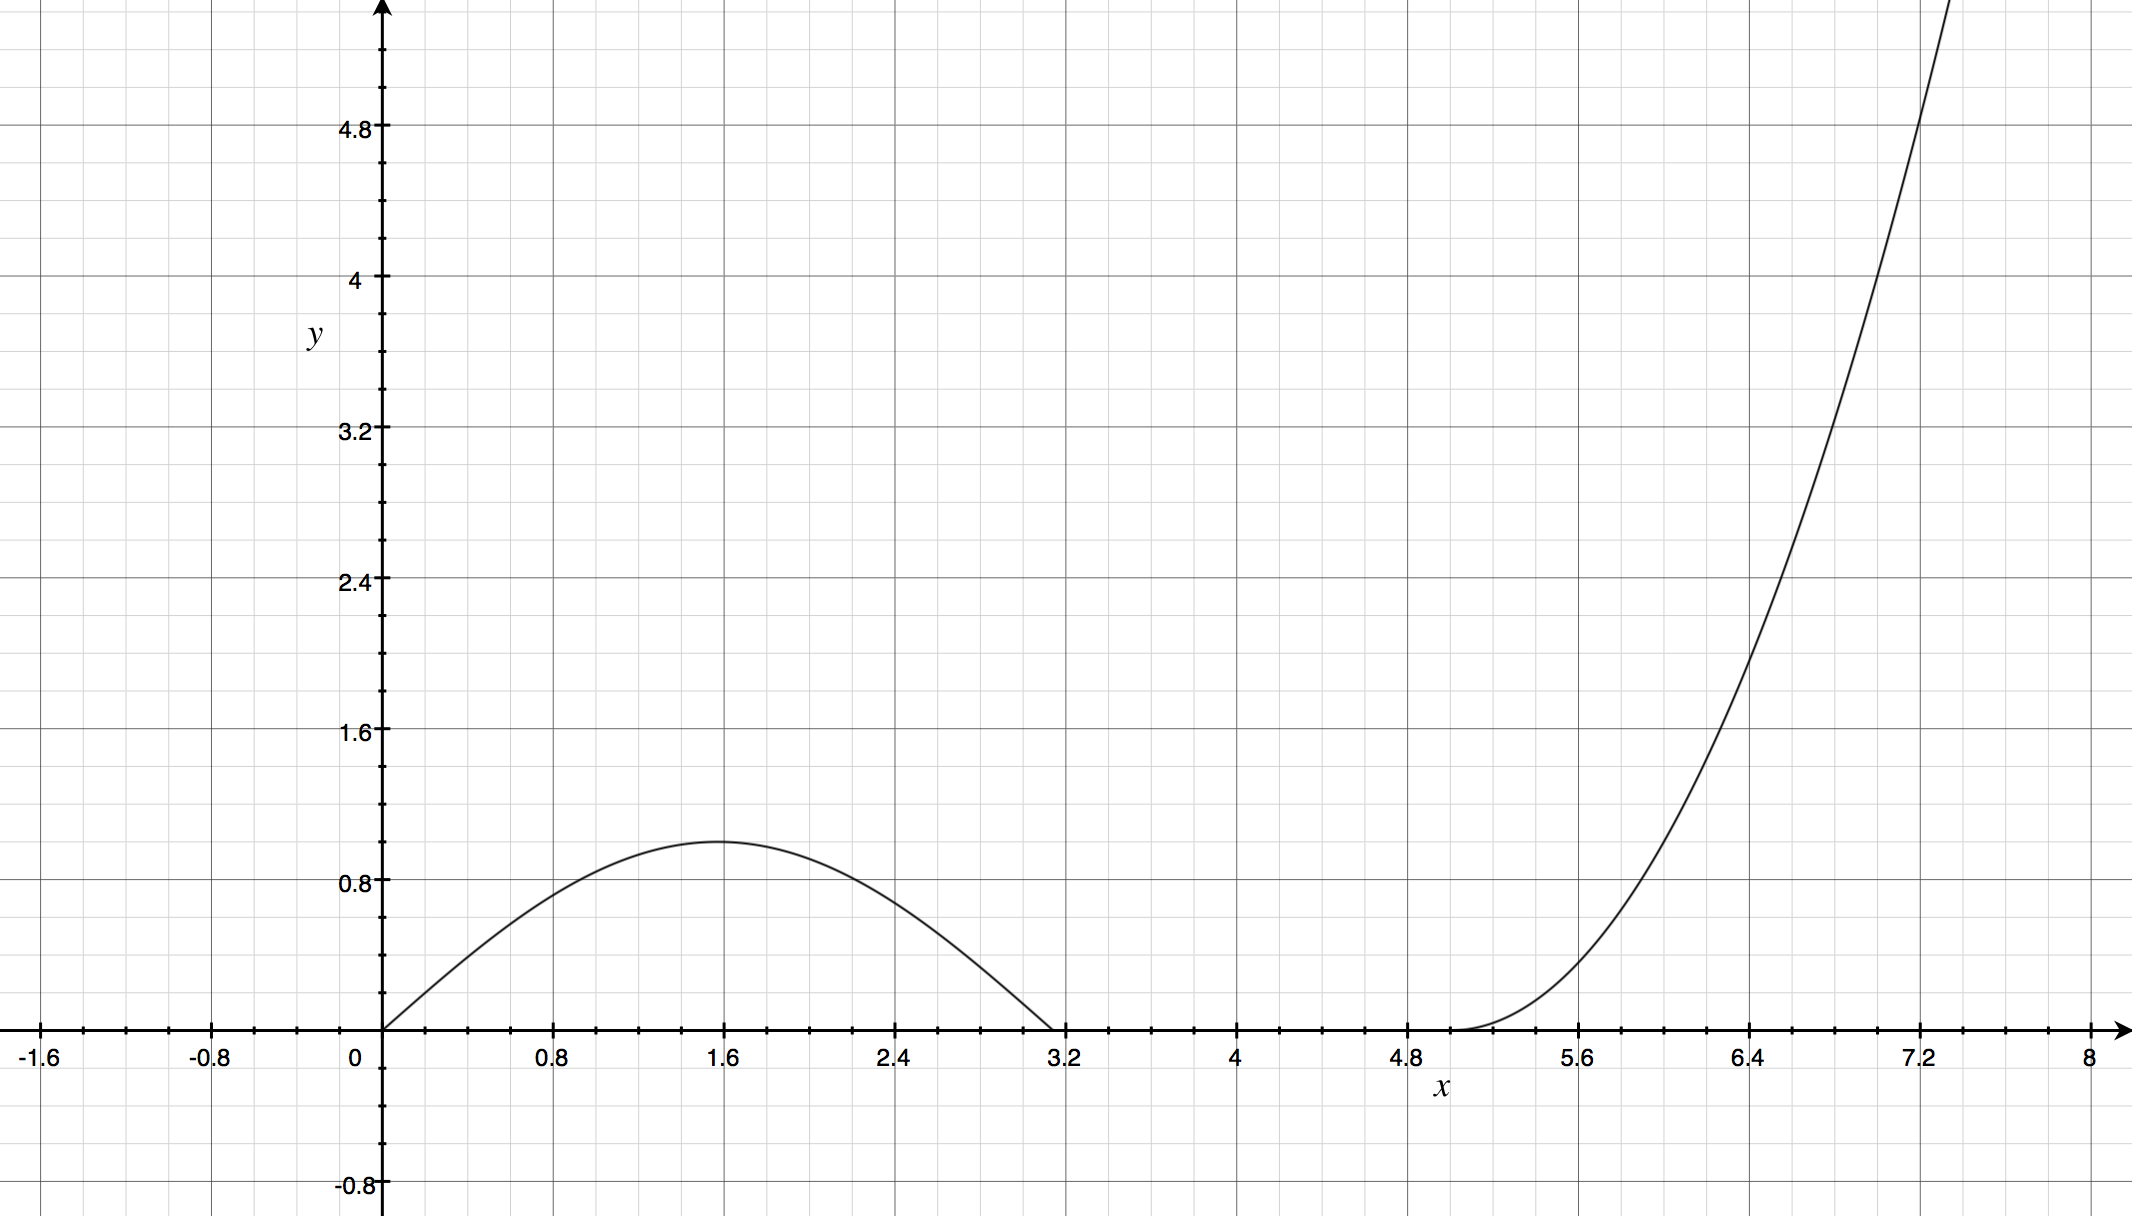
\includegraphics[scale=0.2]{q1graph.png}
\end{center}

\section*{Question 2}

Use the Laplace transform to find the particular solution of the following functions
$$y' + y = \sin(t - 3)u(t - 3) + tu(t - 3) - 3u(t - 3)$$


\noindent Where
\[
 u(t) =
  \begin{cases}
    0 &\text{when } t < 0 \\
    1 &\text{when } t \ge 0
  \end{cases}
\]

\end{document}
